\chapter{Minimalbeispiel 3D-Stereokalibrierung und Szenenrekonstruktion bei Kameras gleicher Auflösung}



\section{Vorgehen: Projektion eines Quaders in zwei verschieden transformierte Kameras}

Um den Mathematischen Vorgang der stereoskopischen Szenenrekonstruktion zu verdeutlichen, wurde ein Minimalszenario erstellt. Für dieses Minimalszenario wurde ein Objekt in diesem Falle ein Quader in ein zuvor Definiertes Weltkoordinatensystem gesetzt. Des Weiteren wurden zwei Kameras in die Szene platziert. Kamera 1 ist von der Lage Deckungsgleich mit dem Weltkoordinatensystem. Kamera 2 wurde verschoben und Rotiert, um so ein anderes Abbild des Objekts auf dem Sensor so produzieren. Für unsere Berechnungen der Szene sind äußere und innere Kameraparameter von uns festgelegt worde. Für eine Szenenrekonstruktion mit realen Bedinungen müssen diese zunächst ermittelt werden, um die aufgezeigten mathematischen Vorgänge anwenden zu können.\\

	Für die Stereokamerakalibrierung wird eine der beiden Kameras relativ zur ersten Kamera um einen Vector \ensuremath{\vec{v}} verschoben und anschließend um einen Winkel \ensuremath{\alpha} um die e2 Achse (vgl. mit Dokumentation Koordinatensysteme) gedreht. 
Für die Rotation um \ensuremath{e_2} gilt folgende Drehmatrix:

\begin{gather}		
R= 
\begin{pmatrix}
\cos(\alpha)&0&\sin(\alpha)\\
0&1&0\\
-\sin(\alpha)&0&\cos(\alpha)
\end{pmatrix}
\end{gather}

Um die Transformationsmatrix \ensuremath{M} welche die Rotation und die Translation beinhaltet zu bekommen werden \ensuremath{R} und \ensuremath{\vec{v}} miteinander verrechnet, hierzu wird aus \ensuremath{\vec{v}} eine Matrix \ensuremath{V} gebildet. 

\begin{gather}
V= 
\begin{pmatrix}
1&0&0&-v_1\\
0&1&0&-v_2\\
0&0&1&-v_3			
\end{pmatrix}\\
M=R^T\cdot V\\
M=		\begin{pmatrix}
\cos(\alpha)&0&-\sin(\alpha)\\
0&1&0\\
\sin(\alpha)&0&\cos(\alpha)
\end{pmatrix} 
\cdot
\begin{pmatrix}
1&0&0&-v_1\\
0&1&0&-v_2\\
0&0&1&-v_3			
\end{pmatrix}\\
M=
\begin{pmatrix}
\cos(\alpha)&0&-\sin(\alpha)&-v_1\cos(\alpha)+v_3\sin(\alpha)\\
0&1&0&-v_2\\
\sin(\alpha)&0&\cos(\alpha)&-v_1\sin(\alpha)-v_3\cos(\alpha)\\
\end{pmatrix}
\end{gather}\\

Die entstandene Matrix \ensuremath{M} beschreibt die Transformation der der Kamera 2 und somit auch die Transformation des Koordinatensystems der Kamera 1 in das Koordinatensystem der Kamera 2.

\begin{minipage}{\linewidth}
	\centering
	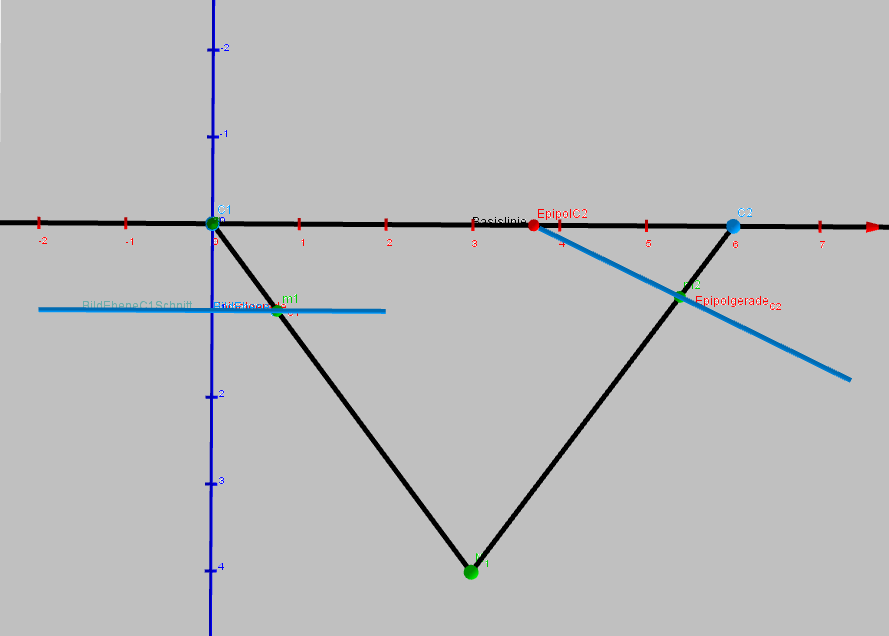
\includegraphics[width=1.\linewidth]{images/TopDownSystem.png}
	\captionof{figure}{Top-Down-Ansicht des entstandenen Aufbaus der Kameras}
\end{minipage}\\ \\

\begin{minipage}{\linewidth}
	\centering
	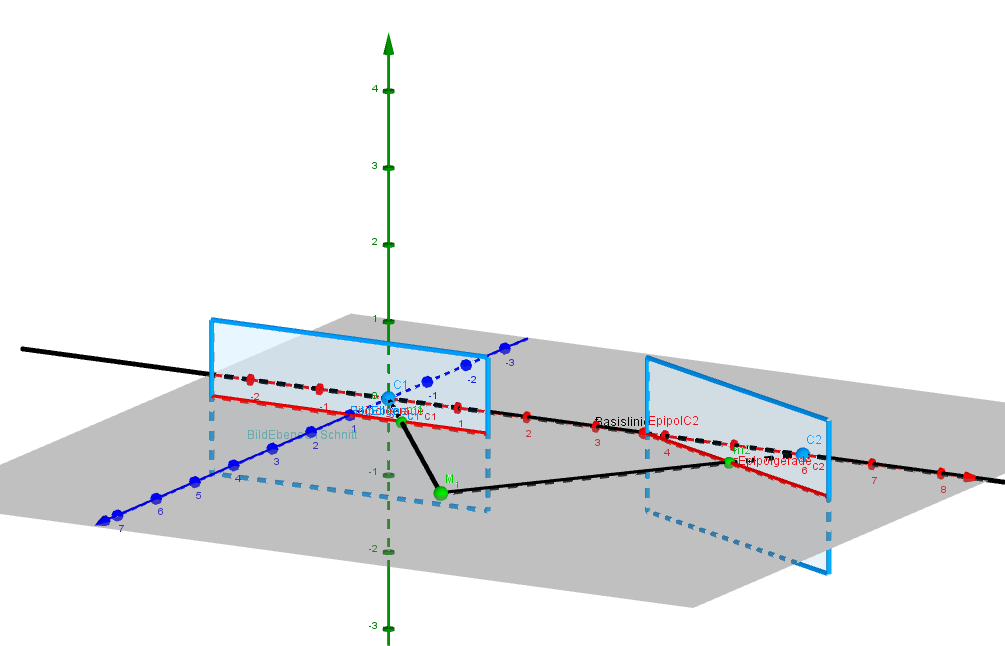
\includegraphics[width=1.\linewidth]{images/3DAnsichSystem.png}
	\captionof{figure}{3D-Ansicht des entstandenen Aufbaus der Kameras}
\end{minipage}\\ \\

%	\subsubsection{Drehung um einen Drehpunkt}	
%	Funktion RotationOfCameraAroundPivotPoint 

\section{Berechnung der Projetkionsmatritzen}

Die Punkte \ensuremath{a,b,c,d,a',b',c',d',d2} in Weltkoordinaten sind bekannt. Die ersten acht Punkte bilden gemeinsam einen Quader, der neunte Punkt ist aus diesem Quader ausgelagert.	
Um die Koordinaten der Punkte in Kamera 1 und Kamera 2 Koordinaten zu Transformieren, muss zusätzlich zur Transformationsmatrix für Kamera2 noch die Abbildungsmatrix \ensuremath{AB1} und \ensuremath{AB2} der jeweiligen Kamera berücksichtigt werden. 

\begin{gather}		
AB1 =
\begin{bmatrix}
\zeta_{K1}&0&0&0\\
0&\zeta_{K1}&0&0\\
0&0&\zeta_{K1}&0\\
0&0&1&0
\end{bmatrix}\\
AB2 =
\begin{bmatrix}
\zeta_{K2}&0&0&0\\
0&\zeta_{K2}&0&0\\
0&0&\zeta_{K2}&0\\
0&0&1&0
\end{bmatrix}
\end{gather}

Um die Projektionsmatrizen \ensuremath{PM1} und \ensuremath{PM2} zu berechnen, bekommt die Matrix \ensuremath{M} noch eine Homogene erweiterung und sieht dann folgendermaßen aus:

\begin{gather}
M=
\begin{bmatrix}
\cos(\alpha)&0&-\sin(\alpha)&-v_1\cos(\alpha)+v_3\sin(\alpha)\\
0&1&0&-v_2\\
\sin(\alpha)&0&\cos(\alpha)&-v_1\sin(\alpha)-v_3\cos(\alpha)\\
0&0&0&1
\end{bmatrix}\\
PM1 = AB1\cdot I_{4x4} \\
PM1 =
\begin{bmatrix}
\zeta_{K1}&0&0&0\\
0&\zeta_{K1}&0&0\\
0&0&\zeta_{K1}&0\\
0&0&1&0
\end{bmatrix}
\end{gather}
\ensuremath{I} ist die Einheitsmatrix, wir gehen davon aus das Kamera 1 weder eine Drehung noch eine Translation beinhaltet und ihr Ursprung sich im Weltkoordinatenurspung befindet.\\


\begin{gather}
PM2 = AB2 \cdot M\\
PM2 =
\begin{bmatrix}
\zeta_{K2} \cos(\alpha)&0&\zeta_{K2} \sin(\alpha)&-\zeta_{K2} (v_1\cos(\alpha)+v_3\sin(\alpha) )&0\\
0&1&0&\zeta_{K2}-v_2&0\\
\zeta_{K2}\sin(\alpha)&0&\zeta_{K2}\cos(\alpha)&-\zeta_{K2}(v_1\sin(\alpha)+v_3\cos(\alpha))\\
0&0&0&0&1
\end{bmatrix}
\end{gather}

\section{Transformation der Weltpunkte in Koordinaten der Koordinatensysteme von beiden Kameras}

	Die 3D-Punkte \ensuremath{a,b,c,d,a',b',c',d',d2}, werden um eine Homogene Komponenten erweitert und mit den Projektionsmatrizen \ensuremath{PM1} und \ensuremath{PM2} verrechnet. Die so neu entstehenden Punktematrix \ensuremath{PK1} mit  \ensuremath{K1a,K1b,K1c,K1d,K1a',K1b',K1c',K1d',K1d2} und \ensuremath{PK2} mit \ensuremath{K2a,K2b,K2c,K2d,\linebreak K2a',K2b',K2c',K2d',K2d2} beschreiben jeweils den selben Quader aus den beiden verschiedenen Kamerakoordinatensystemen.\\

\begin{gather}		
PK1 =		
\begin{bmatrix}
\begin{pmatrix}
\\a\\\\1
\end{pmatrix}&
\begin{pmatrix}
\\b\\\\1
\end{pmatrix}&
\begin{pmatrix}
\\c\\\\1
\end{pmatrix}&
\begin{pmatrix}
\\d\\\\1
\end{pmatrix}&
\begin{pmatrix}
\\a'\\\\1
\end{pmatrix}&
\begin{pmatrix}
\\b'\\\\1
\end{pmatrix}&
\begin{pmatrix}
\\c'\\\\1
\end{pmatrix}&
\begin{pmatrix}
\\d'\\\\1
\end{pmatrix}&
\begin{pmatrix}
\\d2\\\\1
\end{pmatrix}
\end{bmatrix}
\cdot
PM1\\
PK2 =		
\begin{bmatrix}
\begin{pmatrix}
\\a\\\\1
\end{pmatrix}&
\begin{pmatrix}
\\b\\\\1
\end{pmatrix}&
\begin{pmatrix}
\\c\\\\1
\end{pmatrix}&
\begin{pmatrix}
\\d\\\\1
\end{pmatrix}&
\begin{pmatrix}
\\a'\\\\1
\end{pmatrix}&
\begin{pmatrix}
\\b'\\\\1
\end{pmatrix}&
\begin{pmatrix}
\\c'\\\\1
\end{pmatrix}&
\begin{pmatrix}
\\d'\\\\1
\end{pmatrix}&
\begin{pmatrix}
\\d2\\\\1
\end{pmatrix}
\end{bmatrix}
\cdot
PM2
\end{gather}

Die entstanden Koordinaten sehen dann entsprechen Gleichung 16 aus und müssen dann wieder auf eine homogene Form gebracht werden. 

\begin{gather}
aK2 = 
\begin{pmatrix}
x\\y\\\delta z\\\delta
\end{pmatrix}
\leadsto aK2= 
\begin{pmatrix}
\frac{x}{\delta}\\ \frac{y}{\delta}\\ \frac{\delta z}{\delta}\\ \frac{\delta}{\delta}
\end{pmatrix}
\leadsto aK2 =
\begin{pmatrix}
\tilde{x}\\
\tilde{y}\\
z\\
1
\end{pmatrix}
\end{gather}\\

\begin{minipage}{\linewidth}
	\centering
	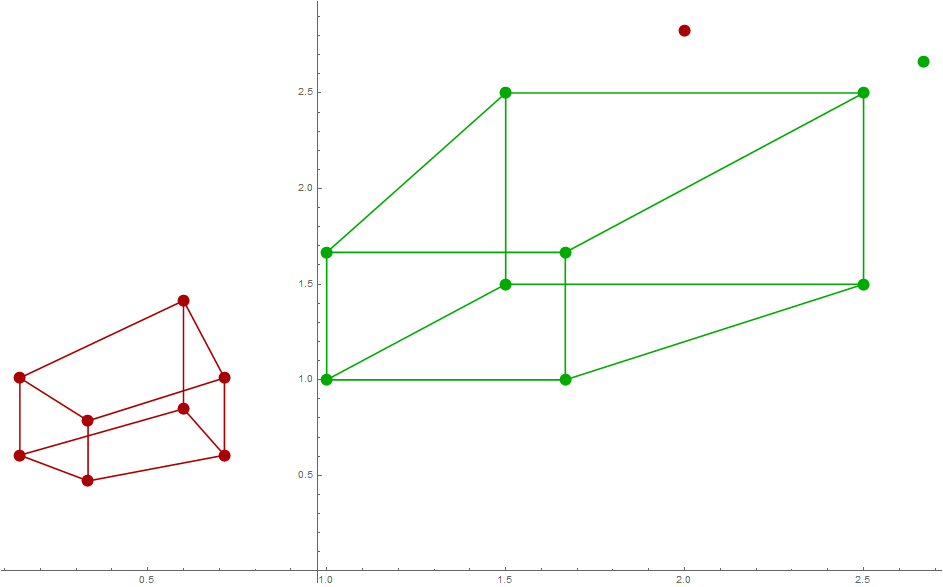
\includegraphics[width=0.8\linewidth]{images/Camer1and2Objects.png}
	\captionof{figure}{Grün zeigt den Quader aus sicht von Kamera 1. Das größere Quadrat sind die vorderen Punkte \ensuremath{a,b,c,d}, das kleinere Quadrat sind die hinteren Punkte \ensuremath{a',b',c',d'}. Rot zeigt denselben Quader aus Sicht vom Kamera 2, wenn diese in +\ensuremath{e_1}-Richtung verschoben und um 45° um \ensuremath{e_2} gedreht wurde}
\end{minipage}\\
\section{Berechnung der projizietrten Punkte auf den beiden Bildebenen}

Um die 3D-Kamerakoordinaten auf die 2D-Bildebene zu Projizieren muss man lediglich die Tiefeninformation der Punkte \ensuremath{PK1} und \ensuremath{PK2} entnehmen und durch die homogene Koordinate ersetzen. Die folgende Gleichung zeigt ein Beispiel dazu 

\begin{gather}
aK2 =
\begin{pmatrix}
\tilde{x}\\
\tilde{y}\\
z\\
1
\end{pmatrix} 
\leadsto aBK2 = 		
\begin{pmatrix}
\tilde{x}\\
\tilde{y}\\
1
\end{pmatrix}
\end{gather}

\section{Umrechnung von Bildebenenkoordinaten in Sensorkoordinaten}
	Für die Umrechnung der Bildebenenkoordinaten \ensuremath{BK1} und \ensuremath{BK2} in Sensorkoordianten, muss der sogenannte Pixelpitch des Sensors bekannt sein. Nehmen wir für unser Beispiel man an wir haben einen PixelPitch von 1. Dann bedeutet dies, dass die Bilebenenkoordinaten in mm 1:1 in die Sensorkoordinaten in Pixel umgesetzt werden können. In der Realität ist dies aber eher selten der Fall. \\
Das Sensorkoordinatensystem wird folgendermaßen beschrieben:

\begin{gather}
K_s = (\vec{u},\vec{v},O_s)\\	
\vec{u} = u_1b_1+u_2b_2\\
\vec{v} = v_1b_1+v_2b_2\\
O_s = O_B+p_1b_1+p_2b_2\\
(\vec{u},\vec{v},O_s)=(b_1,b_2,O_B)\cdot
\begin{bmatrix}
u_1&u_2&p_1\\
v_1&v_2&p_2\\
0&0&1
\end{bmatrix}	\\
M_S = 	
\begin{bmatrix}
u_1&u_2\\
v_1&v_2
\end{bmatrix}
\end{gather}

Stellen wir nun \ensuremath{	\leftidx{_{K_{s}}}{\begin{bmatrix}
			\pi
	\end{bmatrix}}{_{K_{}}}} dar\\

\begin{gather}
\begin{bmatrix}
&&\\
&M^{-1}& -M\begin{pmatrix}p_1\\p_2\end{pmatrix}^{-1}\\
&&\\
0&0&1
\end{bmatrix}
\cdot
\begin{bmatrix}
-\zeta&0&0&0\\
0&-\zeta&0&0\\
0&0&1&0
\end{bmatrix}
=
\begin{bmatrix}
&&&0\\
&-\zeta M^{-1}& -M\begin{pmatrix}p_1\\p_2\end{pmatrix}^{-1}&0\\
&&&\\
0&0&1&0
\end{bmatrix}\\
aSK2 = 
\begin{bmatrix}
&&&0\\
&-\zeta M^{-1}& -M\begin{pmatrix}p_1\\p_2\end{pmatrix}^{-1}&0\\
&&&\\
0&0&1&0
\end{bmatrix} 
\cdot
aBK2
\end{gather}\\

Als Beispiel nehmen wir an wir haben einen Pixelpitch \ensuremath{p} und es gilt \ensuremath{\vec{u} = 1pb_1} und \ensuremath{\vec{v}=2pb_2}. Des Weiteren sei \ensuremath{p_1} =15 und \ensuremath{p_2} = 20.

\begin{gather}
O_s = O_B - \vec{u}-\vec{v} \leadsto O_s = O_B-15b_1-20b_2\\
M_S = \begin{bmatrix}
1&0\\
0&2
\end{bmatrix} \leadsto M^{-1} =
\begin{bmatrix}
\frac{1}{p}&0\\
0&\frac{1}{2p}
\end{bmatrix}\\
\leadsto [\pi]=
\begin{bmatrix}
\frac{\zeta}{p}&0&15&0\\
0&\frac{\zeta}{2p}&20&0\\
0&0&1&0
\end{bmatrix}\\
\end{gather} 



\section{Ermitteln der Fundamentalmatrix mit Hilfe des 8-Point-Algorithms}
	Sind die Sensorkoordinaten berechnet, kann nun die Fundamentalmatrix mit Hilfe des 8-Point-Algorithms ermittelt werden. Für die Fundamentalmatrix benötigen wir mindestens sieben Punktekorrespondenzen. Mit sieben Punkten bekommen wir als Lösung des 8-Point-Algorithm zwei linear unabhängige Kerne als Lösung der Koeffizientenmatrix mit welchen weiter verfahren werden muss (Mehr dazu später). Hartley und Zisserman schlagen vor, dass sich zur Sicherheit am besten neun Punkte eigenen. Zu beachten ist nämlich, dass wenn die Punkte in sofern voneinander abhängen, dass immer 2 Punkte auf der selben Epipolarlinie liegen, verliert unsere Koeffizientenmatrix an Rang und wir bekommen  wie bei den sieben Punkten zwei Lösungen für den Kern. Aufgrund dessen haben wir einen neunten Punkt\ensuremath{d2} zu unserem Quader hinzugefügt, welcher nicht Gefahr läuft auf der selben Epipolarlinien wie ein anderer Punkt zu liegen.\\

Wir haben also nun unsere 9 Punkte auf dem Sensor der Kamera 1 \ensuremath{SK1} und dem Sensor der Kamera 2 \ensuremath{SK2}. Die Fundamentalmatrix ist definiert als

\begin{gather}
x'^T F x =0
\end{gather}

Die Fundamentalmatrix ist eine 3x3-Matrix mit Rang 2. Um sie zu ermitteln muss zunächst eine Koeffizientenmatrix nach folgendem Schema erstellt werden: 

\begin{gather}
F=\begin{bmatrix}
f_{11}&f_{122}&f_{13}\\
f_{21}&f_{22}&f_{23}\\
f_{31}&f_{32}&f_{33}
\end{bmatrix}\\
\begin{pmatrix}
x'_n&y'_n&1
\end{pmatrix} 
\cdot
\begin{bmatrix}
f_{11}&f_{122}&f_{13}\\
f_{21}&f_{22}&f_{23}\\
f_{31}&f_{32}&f_{33}
\end{bmatrix}
\cdot
\begin{pmatrix}
x_n\\y_n\\1
\end{pmatrix} =0\\
f_{11}x_nx'_n+f_{12}y_nx'_n+f_{13}x'_n+f_{21}x_ny'_n+f_{22}y_ny'_n+f{23}y'_n+f_{31}x_n+f_{32}y_n+f_{33} =0\\
(x_nx'_n,y_nx'_n,x'_n,x_ny'_n,y_ny'_n,y'_n,x_n,y_n,1)\cdot f =0\\
\begin{bmatrix}
x_1x'_1&y_1x'_1&x'_1&x_1y'_1&y_1y'_1&y'_1&x_1&y_1&1\\
x_2x'_2&y_2x'_2&x'_2&x_2y'_2&y_2y'_2&y'_2&x_2&y_2&1\\
.&.&.&.&.&.&.&.&.\\
.&.&.&.&.&.&.&.&.\\
.&.&.&.&.&.&.&.&.\\
x_nx'_n&y_nx'_n&x'_n&x_ny'_n&y_ny'_n&y'_n&x_n&y_n&1
\end{bmatrix}
\cdot 
\begin{pmatrix}
f_{11}\\f_{12}\\f_{13}\\f_{21}\\f_{22}\\f_{23}\\f_{31}\\f_{32}\\f_{33}
\end{pmatrix}
= 0
\end{gather}

Der Kern und alle seine Vielfache sind Lösungen für die Fundamentalmatrix. Um den Kern aus der Koeffizientenmatrix zu berechnen wird der null-space oder auch Nullraum ermittelt. der null-space beschreibt denjenigen Vektor, welcher durch multiplizieren mit der Koeffizientenmatrix gleich den Nullvektor ergibt.

\begin{gather}
A\cdot f 
\end{gather} \\

Also Kern bekommt man in diesem Fall eine Liste mit Einträgen. 
Diese neun Einträge ergeben dann die Werte der 3x3-Fundamentalmatrix. 


\section{Berechnen der Epipole und Epipolargeraden mit der Fundamentalmatrix}
	Mit Hilfe der Fundamentalmatrix und dem Wissen über die Epipolargerometrie, kann man die Epipole \ensuremath{e} und \ensuremath{e'}, sowie die Epilolargeraden \ensuremath{l} und \ensuremath{l'} ermitteln. Im ersten Abschnitt wird die ermittlung mit Hilfe der Fundamentalmatrix aufgezeigt und in Kapitel 1.2.1 wird nochmal drauf eingegangen und aufgezeigt, wie sich die Epipolarlinien und Epipole geometrisch Konstruieren lassen.\\

Mit der Fundamentalmatrix lassen sich die Epipolargerade folgendermaßen berechnen

\begin{gather}
l' = F \cdot x\\
l = F^T \cdot x'
\end{gather}\\

\ensuremath{l'} ist die zu \ensuremath{x} korrespondierende Epipolargerade. \ensuremath{l} ist die zu \ensuremath{x'} korrespondierende Epipolargerade. Zu Berechnung des Epipols \ensuremath{e} muss der Rechte Null-Space von F ermitteln werden und für den Epipol \ensuremath{e'} brauchen wir den linken Null-Space. Um diesen zu bekommen ermitteln wir wie bekannt den Kern aber diesmal von \ensuremath{F^T} statt \ensuremath{F}. Die Abbiludng 4 zeigt, dass Ergebnis.

\begin{minipage}{\linewidth}
	\centering
	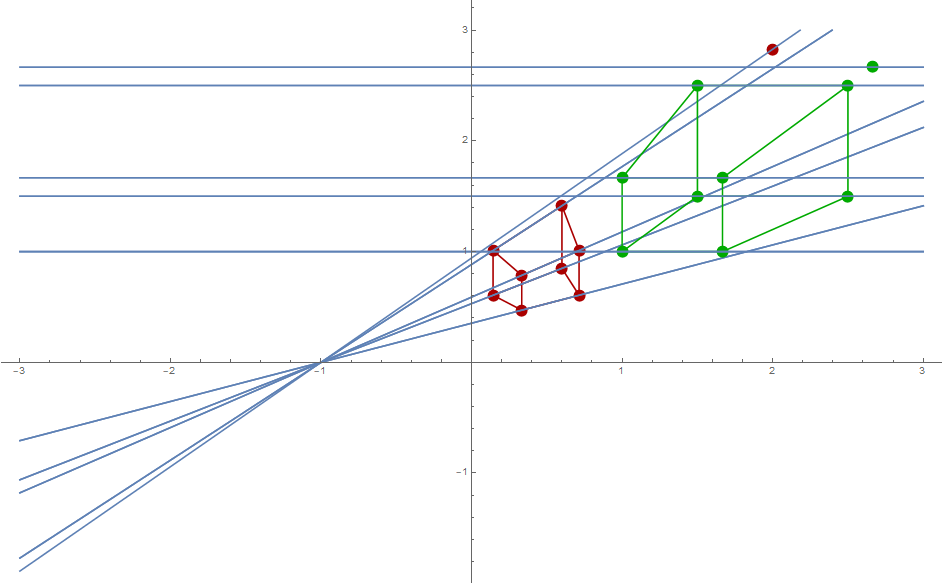
\includegraphics[width=1.\linewidth]{images/Epipole_Epipollinien.png}
	\captionof{figure}{Die blauen Geraden zeigen die jeweiligen Epipolargeraden. Die vom roten Quader schneiden sich bei -1 im Epipol. Die Epipolargeraden vom grünen Quader schneiden sich im Epipol im Unendlichen}
\end{minipage}\\ \\

\subsection{Konstruktion der Epipole und der Epipolgeraden auf Grundlage der Epipolargeometrie}
	Die Vorgehensweise zur Ermittlung der Epipole und der Epipolgeraden ist zwar schnell aber zur verdeutlichung der geometrischen Beziehungen untereinander wird hier nochmal eine rein geoemtrische Konstruktion der Epipole und der Epipolargeraden aufgezeigt. Im nachfolgenden Beispiel wird der Epipol \ensuremath{e'} geometrisch konstruiert. \\

Vorbedinungen: Wir berechnen alles in Weltkoordinaten, hierzu muss sichergestellt sein dass alle Werte im Weltkoordinaten angegeben sind oder gegebenenfalls noch umgerechnet werden müssen. \\
Für die Konstruktion der Epipole brauchen wir folgendes:
\begin{itemize}
	\item Die Basisgerade zwischen den Kamerazentren, welche sich un unserem Beispiel mit dem Ursprung des Kamerakooridnatensystems decken
	\item einen Punkt auf der Bildebne in Bildebenenkoordinaten (mm), nicht in Sensorkoordinaten, der Kamera 2 ,welcher Weltkooridnaten umgerechnet werden muss
	\item Die Bildebene der Kamera 2 
\end{itemize}

Für unser Beispiel nennen wir das Kamerazentrum der Kamera 1 \ensuremath{O_c} und das Kamerazentrum der Kamera 2 \ensuremath{O2_c} (vgl mit vorherigen Dokumentationen). Wir erstellen auf Grundlage dieser zwei bekannten Punkte eine Gerade, welche durch die beiden Kamerazentren geht

\begin{gather}
BaseLine = Oc_2 + t\cdot (Oc_2-O_c)
\end{gather}

Um den Epipol zu ermitteln müssen wir nun den Schnittpunkt der Gerade \ensuremath{BaseLine} mit der Bildebenen \ensuremath{ImagePlane'} der Kamera 2 finden. Also müssen wir jetzt die Ebenengleichung der Bildebenen aufstellen. Am einfachsten ist es wenn man zunächst die Normalenform aufstellt.\\

\begin{gather}
\vec{n_0}\cdot[\vec{x}-\vec{a}]
\end{gather}

Nehmen wir das bereits bekannte Beispiel von vorhin, in welchem die Kamera 2 entlang der positiven \ensuremath{e_1} verschoben und um 45° um die \ensuremath{e_2}-Achse gedreht wurde, so ist der normalen Vektor der Bildebene aus sicht der Weltkoordinaten \ensuremath{\vec{n_0} = \begin{pmatrix}
		-1\\0\\-1
\end{pmatrix}}. Für die Ebene brauchen wir nun noch einen Punkt welcher auf ihr liegt. In unserem Beispiel nehmen wir als Aufpunkt \ensuremath{\vec{a}} den Punkt \ensuremath{a} in Bildkoordinaten \ensuremath{aBK2} der 2. Kamera und rechnen diesen in Weltkoordinaten zurück. Wir brauchen also die nicht-transponierte Rotation \ensuremath{R} welche lautet:

\begin{gather}
R=\begin{pmatrix}
\cos{\alpha}&0&\sin{\alpha}\\
0&1&0\\
-\sin{\alpha}&0&\cos{\alpha}
\end{pmatrix}
\end{gather}

Des Weiteren brauchen wir den verschiebe Vektor \ensuremath{\vec{v} = \begin{pmatrix}
		v_1\\v_2\\v_3
\end{pmatrix}},welcher mit \ensuremath{R} verrechnet wird.


\begin{gather}
\begin{pmatrix}
\cos{\alpha}&0&\sin{\alpha}\\
0&1&0\\
-\sin{\alpha}&0&\cos{\alpha}
\end{pmatrix}
\cdot
\begin{pmatrix}
v_1\\v_2\\v_3
\end{pmatrix}
=
\begin{pmatrix}
v_1\cos{\alpha}+v_3\sin{\alpha}\\
v_2\\
-v_1\sin{\alpha}+v_3\cos{\alpha}
\end{pmatrix}\\
\leadsto D =
\begin{bmatrix}
\cos{\alpha}&0&\sin{\alpha}&v_1\cos{\alpha}+v_3\sin{\alpha}\\
0&1&0&v_2\\
-\sin{\alpha}&0&\cos{\alpha}&-v_1\sin{\alpha}+v_3\cos{\alpha}\\
0&0&0&1
\end{bmatrix}
\end{gather}\\

Matrix \ensuremath{D} wird dann mit Punkt \ensuremath{aBK2} multipliziert und wir bekommen den Punkt \ensuremath{aBK2} in Weltkoordinaten \ensuremath{aWK2}. Die Normalengleichung ist somit komplett aufgestellt. um auf die Koordinatengleichung zu kommen werden die Skalare einfach ausmultipliziert. 

\begin{gather}
\vec{n_0}\cdot \vec{x} - \vec{n_0}\cdot \vec{a}\\
ImagePlane:ax+by+cz+d = 0
\end{gather}

Danach wird die Geradengleichung \ensuremath{BaseLine} in die Ebenengleichung \ensuremath{ImagePlane} eingesetzt und es wird ein Wert für \ensuremath{t} ermittelt. Dieser wird wiederum in die Geradegleichung eingesetzt und das Ergebnis ist der Epipol \ensuremath{e'}, jedoch noch in Weltkoordinaten. Dieser muss dann nach dem selben Scheme wie am Anfang gezeigt von Welt in Sensorkoordianten umgerechnet werden. 

\begin{gather}
e'_{Sensor}=PM2.e'_{Welt}
\end{gather}

Die dritte Zeile kann dadurch dass wir eine 1 zu 1 umsetzung von Bildebenenkoordinaten (mm) auf Sensorkoordinaten (Pixel) haben einfach rausgestrichen und durch die vierte Zeile ersetzt werden.


\section{Ermitteln der Essentiellen Matrix über die Fundamentalmatrix}
	Nachdem nun die Fundamentalmatrix haben und Epipole und Epipolarlinien bestimmt sind, wollen wir mit Hilfe der Fundamentalmatrix die Essentielle Matrix bestimmen, aus welcher wir die externen Kameraparameter extrahieren wollen.

\begin{gather}
\hat{x}'^T.E.\hat{x} = 0
\end{gather}\\ 

In unserem Minimalbeispiel sind innere und äußere Kameraparameter ja bereits bekannt, somit können wir leichter erkennen ob unsere Ergebnisse mit der den Vordefinierten Werten übereinstimmen. Wir gehen also jetzt davon aus, dass wir die externen Kameraparameter noch nicht kennen. Wir kennen die Fundamentalmatrix \ensuremath{F} und wir kennen die inneren Kameraparameter \ensuremath{AB1} und \ensuremath{AB2} (vgl. Kapitel 1.2).
Anzumerken ist noch, dass wir für die Essentielle Matrix nicht die Sensorkoordinaten, sondern die Bildebenenkoordinaten betrachten, welche zuvor auch noch normiert werden müssen. In Gleichung 46 ist dies durch \ensuremath{\hat{x}'} und \ensuremath{\hat{x}} gekennzeichnet. Der Normierungsvorgang sieht folgendermaßen aus.	

\begin{gather}
aK2 = PM2\cdot a\\
aK2 = AB2[R|t]\\
AB2^{-1}\cdot aK2 = AB2^{-1}\cdot AB2[R|t] a\\
\hat{aK2} = [R|t]\\
[R|t]\, \widehat{=} \, M
\end{gather}

\ensuremath{\hat{aK2}} beschreibt die normierte Koordinate von \ensuremath{aK2}. Um die Essentielle Matrix aus der Fundamentalmatrix herzuleiten benutzen wir folgende Formel.

\begin{gather}
E = AK2^T.F.AK1
\end{gather}

Die Lösung dieser Gleichung gibt uns eine Mögliche Lösung der Essentiellen Matrix. Vergleichen wir das Ergebnis mit dem Ergebnis welches wir bekommen, wenn die Essentielle Matrix über den 8-Point-Algorithm berechnet wurde, so kann man erkennen dass sie Vielfache voneinander sind.

\subsection{Ermitteln der Essentiellen Matrix mit normierten Bildkoordinaten und dem 8-Point-Algorithm}

	Im vorherigen Abschnitt haben wir bereits die normierten Bildebenenkoordinaten berechnet. Um die essentielle Matrix mit dem 8-Point-Algorithm zu bestimmen, verfährt genau so wie bei der Bestimmung der Fundamentalmatrix nur verwendet man statt den Sensorkoordinaten die normierten Bildebenenkoordinaten.\\ (vgl Hartley and Zisserman, O. Schreer)

Um herauszufinden, ob die errechnete Matrix den Kriterien einer Essentiellen Matrix entspricht gilt folgendes zu überprüfen.

\begin{itemize}
	\item Zwei der Singulärwerte und der Eigenwerte der Essentiellen Matrix müssen gleich und von null verschieden sein.
	\item Die Quadratwurzel der Eigenwerte muss die Singulärwerte ergeben
	\item Der Rang der Matrix muss zwei sein
\end{itemize}

\section{Ermitteln der exterenen Kameraparameter mit Hilfe der Essentiellen Matrix}

	
Um nun die äußeren Kameraparameter zu bestimmen, muss zunächst die Essentielle Matirx \ensuremath{E} mit Hilfe der Singulärwertszerlegung zerlegt werden. Das Ergebnis sind drei Matrizen der Form 

\begin{gather}
E = U\Sigma V^T
\end{gather}

Zu Beachten ist dass die Essentielle Matrix so angepasst werden muss dass am besten für \ensuremath{\Sigma} gilt:

\begin{gather}
\Sigma = diag(1,1,0)
\end{gather}

Mit angepasst ist damit gemeint, dass man das Vielfache des Kerns der Essentiellen Matrix nimmt, so dass die Singulärwerte \ensuremath{diag(1,1,0)} werden.

Wir wissen dass:

\begin{gather}
E=[t]_xR\\
S =[t]_x\\
E=SR
\end{gather}

Zur Unterstüzung der Berechnung der externen Kameraparameter nehmen wir die Matrizen \ensuremath{W} und \ensuremath{Z} zu Hilfe

\begin{gather}
W = \begin{pmatrix}
0&-1&0\\
1&0&0\\
0&0&1
\end{pmatrix} \;\;\;
Z=
\begin{pmatrix}
0&1&0\\
-1&0&0\\
0&0&0
\end{pmatrix}
\end{gather}

Mit dem Ergebnis der SVD von \ensuremath{E} lassen sich nun jeweils zwei Ergebnisse für S und R finden:	

\begin{gather}
S_1 = -UZU^T \;\;\;\; R_1 = UW^TV^T\\
S_2 = UZU^T \;\;\;\; R_2 = UWV^T
\end{gather}\\

Um sicher zu gehen, dass es sich bei \ensuremath{R_1} und \ensuremath{R_2} auch um Rotationen handelt, kann man folgende Proben durchführen. Zum einen muss \ensuremath{R\cdot R^T=I_{3x3}} sein. \ensuremath{I_{3x3}} bezeichnet in diesem Fall eine 3x3-Einheitsmatrix. Des Weiteren kann man überprüfen, ob die Determinante \ensuremath{det(R_1) = 1} ist. Nun müssen wir aus den 3x3-Matrizen \ensuremath{S_1} und \ensuremath{S_2} noch das fehlende \ensuremath{t} rausfiltern. Wir wissen:

\begin{gather}
St = [t]_x \cdot t = t \times t
\end{gather} 

Daraus kann man schließen, dass \ensuremath{t} = dem Null-Space von \ensuremath{S_1} und \ensuremath{S_2} ist. Der Null-Space beider Matrizen \ensuremath{S_1} und \ensuremath{S_2} ist der selbe. Die externen Kamerparameter lassen sich wie gesagt nur bis zu einem Skalierungsfaktor genau berechnen. Dass soll heißen, ist der \ensuremath{t} der Null-Space von \ensuremath{S_1} und \ensuremath{S_2}, so ist auch das Vielfache \ensuremath{\lambda t} eine gültige Lösung für t. Letzten Endes haben wir für die externen Kameraparameter vier verschiedene Lösungen. 

\begin{gather}
PM2 = [UWV^T|+\lambda t] \;\;\; or \;\;\;[UW^TV^T|+\lambda t]\\
or\;\;\; [UWV^T|-\lambda t] \;\;\; or \;\;\;[UW^TV^T|-\lambda t]
\end{gather}
\section{Punkterekonstruktion durch Triangulation}
\subsection{Rektifizierung}